\documentclass[margin=2cm]{standalone}
\usepackage{tikz}
\usepackage{tkz-euclide}
\begin{document}
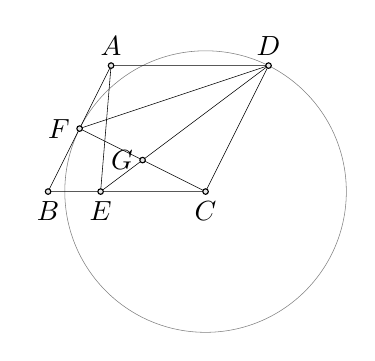
\begin{tikzpicture}
    \tkzDefPoints{0.8/1.6/A, 0/0/B, 2/0/C, 2.8/1.6/D}
    \tkzInterLC(A,B)(C,D)
    \tkzDefPointOnLine[pos=.45](A,B)
    \tkzGetPoints{F}{F'}
    \tkzDrawCircle(C,D)
    %\tkzDrawPoints(F,F')
    %\tkzLabelPoints[left](F,F')
    \tkzDrawPolygon(A,B,C,D)
    \tkzDefPointBy[reflection = over D--F](A)%note有误
    \tkzGetPoint{G}
    \tkzInterLL(D,G)(B,C)
    \tkzGetPoint{E}
    \tkzDrawSegments(D,F C,F A,E D,E)
    \tkzDrawPoints(A,B,C,D,E,F,G)
    \tkzLabelPoints[above](A,D)
    \tkzLabelPoints[below](B,C,E)
    \tkzLabelPoints[left](F,G)
\end{tikzpicture}
\end{document}